% Chapter 3

\chapter{Diseño e implementación} % Main chapter title

\label{Chapter3} % Para referenciar este capítulo: \ref{Chapter3}

En el presente capítulo se describen el diseño y la implementación del sistema. Se presenta la arquitectura general y la distribución del cómputo entre el comercio y la nube. Luego se detalla cada capa: la captura de los pedidos, la conectividad entre los componentes, el procesamiento y la persistencia, la interfaz de usuario y las medidas de seguridad. En cada sección se exponen los problemas encontrados, los criterios adoptados y la justificación de las decisiones tomadas.

%----------------------------------------------------------------------------------------
%	SECTION 1
%----------------------------------------------------------------------------------------

\section{Arquitectura del sistema}
\label{sec:arquitectura}

El sistema se organizó en tres capas funcionales. La capa de captura y comunicación recibe los mensajes del canal de mensajería y los prepara para su interpretación. La capa de procesamiento inteligente interpreta el contenido, lo estructura contra el catálogo del comercio y lo persiste. La capa de interacción local e impresión ejecuta la actuación física sobre la impresora del negocio. En la figura \ref{fig:arquitectura_sistema} se presentan las tres capas, sus componentes y el flujo de datos extremo a extremo.

\begin{figure}[htbp]
  \centering
  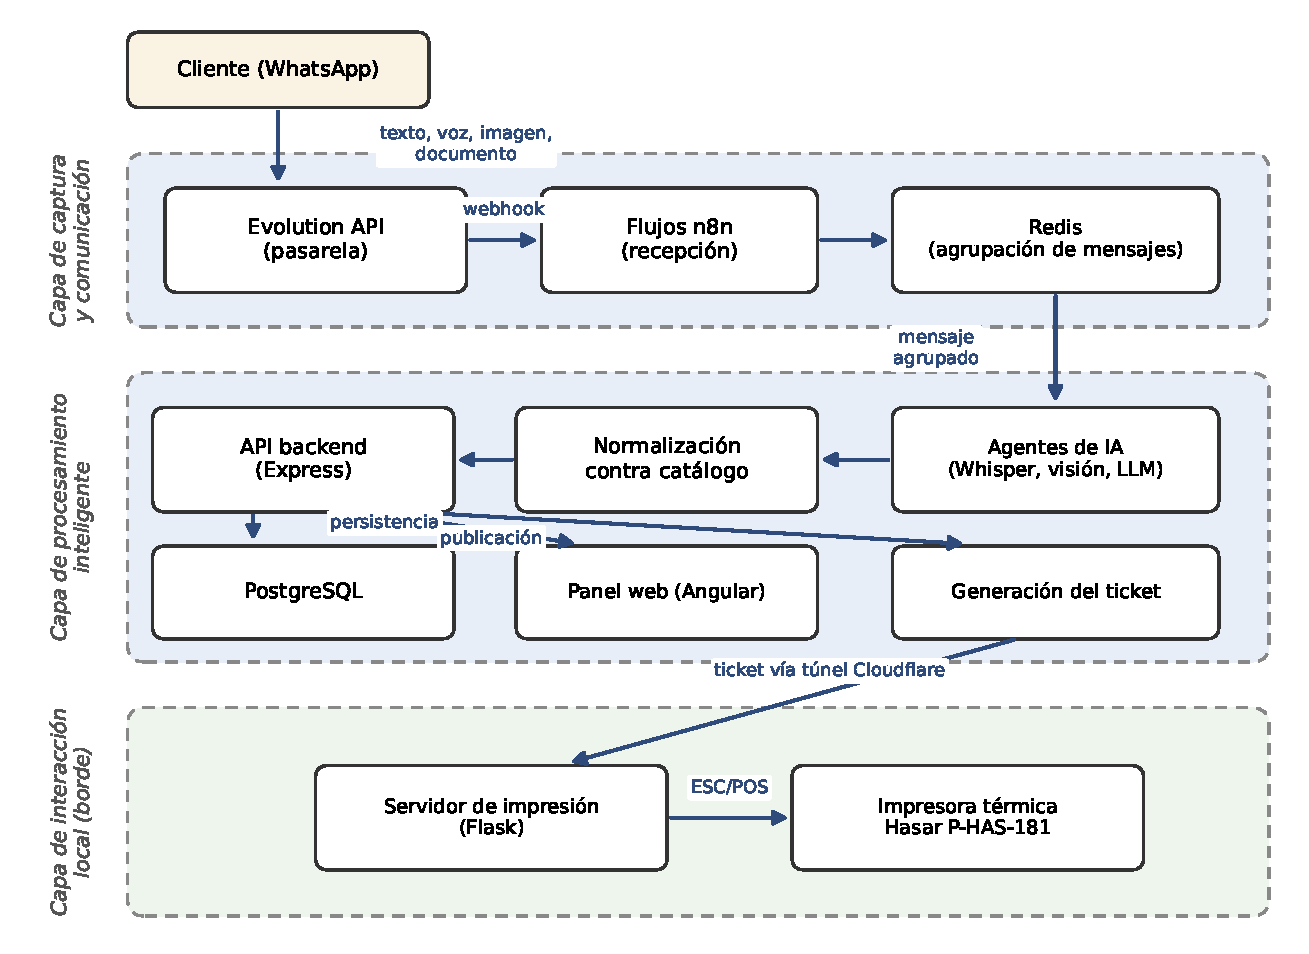
\includegraphics[width=\textwidth]{Figures/arquitectura_sistema.pdf}
  \caption{Arquitectura del sistema en tres capas.}
  \label{fig:arquitectura_sistema}
\end{figure}

\subsection{Criterio de distribución del cómputo}
\label{subsec:criterio_distribucion}

El criterio rector del diseño fue asignar cada tarea al lugar de ejecución que mejor equilibra latencia, disponibilidad y costo. Las tareas de mayor demanda de procesamiento son la transcripción de voz, la lectura de imágenes y la estructuración mediante modelos de lenguaje. Todas ellas se delegaron a servicios en la nube, donde la capacidad de cómputo resulta elástica y los modelos se consumen bajo demanda. Ejecutarlas sobre el equipo del comercio habría exigido una inversión en hardware incompatible con las restricciones económicas del proyecto.

La actuación crítica del negocio es la impresión del ticket que habilita el armado del pedido. Esa tarea se resolvió en el borde, sobre el servidor local del comercio. La decisión responde a tres motivos. El primero es la latencia: la orden de impresión recorre un único salto desde el servidor local hasta la impresora. El segundo es la independencia del canal: la impresora nunca se expone a Internet, sino que queda detrás de un servicio local que actúa como intermediario. El tercero es la continuidad operativa: el personal puede reimprimir un pedido ya recibido desde el panel sin que intervengan los modelos de inteligencia artificial.

\subsection{Organización del código}
\label{subsec:organizacion_codigo}

El código fuente se organizó en cuatro módulos independientes, que se corresponden con los componentes de la arquitectura:

\begin{itemize}
  \item \code{api/}: la interfaz de programación de aplicaciones (API) y la lógica de pedidos, implementadas con Node.js, Express y TypeScript sobre el mapeador objeto-relacional (ORM, del inglés \textit{Object-Relational Mapping}) Prisma.
  \item \code{web/panel/}: el panel web de control, desarrollado con Angular.
  \item \code{n8n/}: los flujos de automatización que orquestan la recepción y la interpretación de los pedidos.
  \item \code{print\_server/}: el servidor de impresión que se ejecuta en el nodo de borde, implementado con Flask.
\end{itemize}

Esta separación permite desplegar, actualizar y probar cada módulo por separado. La API y el panel se comunican solo a través de recursos HTTP, sin dependencias de código compartido, de modo que un cambio en la interfaz no obliga a modificar el servidor.

\subsection{Entorno de desarrollo}
\label{subsec:entorno_desarrollo}

El desarrollo planteó una dificultad práctica: la impresora se encuentra en el comercio y permanece en uso durante el horario comercial, por lo que no resultaba viable ensayar contra el equipo real cada modificación del flujo.

La solución adoptada fue una versión simulada del servidor de impresión. Ese componente expone el mismo recurso y acepta el mismo formato de petición que el servidor real, pero en lugar de enviar el ticket a la impresora lo registra en la consola. El archivo de composición de contenedores del entorno de desarrollo levanta la API, el panel y esa versión simulada, y dirige las peticiones de impresión hacia ella de forma automática.

El resultado fue un entorno de desarrollo completo, reproducible en cualquier equipo y sin dependencia del hardware del comercio. La sustitución se resuelve por configuración, sin cambios en el código de la API, lo que garantiza que el componente ejercitado durante las pruebas sea el mismo que opera en producción.

\subsection{Flujo de datos extremo a extremo}
\label{subsec:flujo_extremo}

El recorrido de un pedido comprende las siguientes etapas. El cliente envía uno o varios mensajes por WhatsApp. La pasarela Evolution API los entrega al flujo de n8n mediante una notificación automática. El flujo clasifica cada mensaje según su tipo y aplica el procesamiento correspondiente hasta obtener texto plano. Ese texto se acumula en una lista temporal en Redis, asociada al teléfono del cliente, y se agrupa con los mensajes contiguos del mismo remitente. El conjunto agrupado se entrega al agente de inteligencia artificial junto con el catálogo vigente de productos y unidades. El agente devuelve el pedido estructurado. La API lo valida, resuelve los precios aplicables, lo persiste y solicita la impresión. El servidor local recibe el ticket a través del túnel seguro y lo envía a la impresora. En paralelo, el pedido queda disponible en el panel web para su seguimiento.

%----------------------------------------------------------------------------------------
%	SECTION 2
%----------------------------------------------------------------------------------------

\section{Capa de captura y comunicación}
\label{sec:capa_captura}

Esta capa recibe los mensajes de los clientes y los convierte en un texto único, listo para su interpretación. Constituye la entrada del sistema y concentra buena parte de su complejidad, porque debe absorber la heterogeneidad del canal.

\subsection{Recepción de los mensajes}
\label{subsec:recepcion}

La recepción se resolvió mediante el mecanismo de notificaciones automáticas de la pasarela Evolution API. Ante cada mensaje entrante, la pasarela emite una petición HTTP hacia el punto de entrada del flujo de n8n. El primer nodo del flujo normaliza la estructura del mensaje recibido y extrae los datos relevantes: el teléfono del remitente, su nombre de perfil, el identificador del mensaje, el tipo de contenido y la marca temporal.

El teléfono cumple una función central en el diseño, ya que opera como identificador natural del cliente a lo largo de todo el flujo. Se utiliza como clave de agrupación de mensajes, como clave de sesión del agente y como criterio de búsqueda del cliente en la base de datos, donde el campo correspondiente tiene restricción de unicidad. La elección resultó natural para el dominio: el número de teléfono es estable, lo provee el propio canal sin intervención del cliente y no requiere ningún registro previo.

El nombre de perfil de WhatsApp, en cambio, resultó insuficiente para identificar al cliente en el negocio. Muchas personas configuran un apodo o dejan el campo vacío, y el comercio conoce a sus clientes por su nombre real o por su razón social. Por ese motivo, el flujo complementa la identificación con una consulta a la agenda de contactos asociada al comercio, y la base de datos conserva un campo propio con el nombre que el personal administra desde el panel.

\subsection{Clasificación y procesamiento por tipo de contenido}
\label{subsec:clasificacion}

Un mismo pedido puede llegar como texto libre, como uno o varios mensajes de voz, como una fotografía de una lista manuscrita, como una captura de una planilla o como un documento adjunto. El flujo resuelve esa diversidad con un nodo de derivación que evalúa el tipo de contenido y envía el mensaje a la rama correspondiente. En la figura \ref{fig:flujo_captura} se muestra el procesamiento completo de esta capa.

\begin{figure}[htbp]
  \centering
  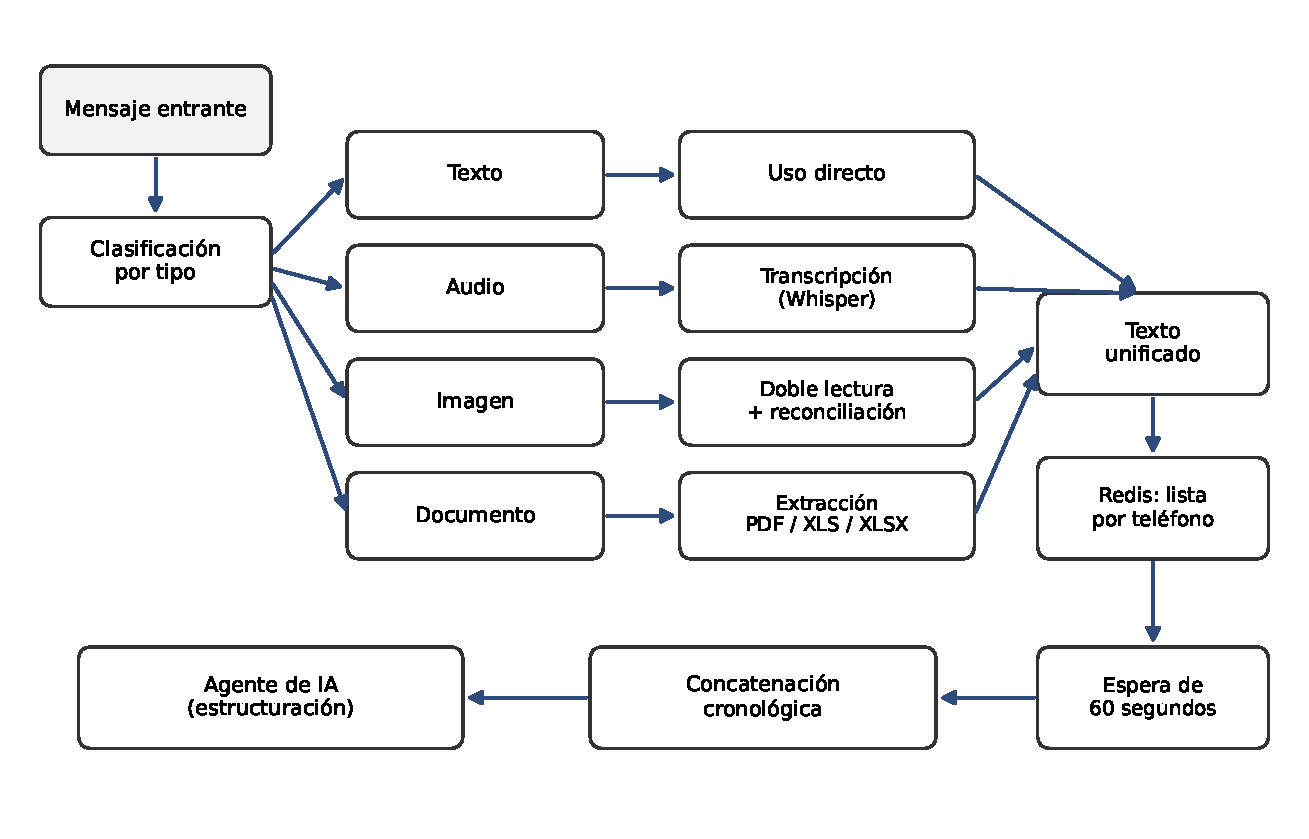
\includegraphics[width=\textwidth]{Figures/flujo_captura.pdf}
  \caption{Procesamiento de la capa de captura, desde el mensaje entrante hasta el texto agrupado.}
  \label{fig:flujo_captura}
\end{figure}

Los mensajes de texto se emplean de forma directa. Los mensajes de voz y las imágenes requieren un paso previo de descarga: la pasarela entrega el contenido multimedia codificado en base64, que luego se convierte en un archivo binario antes de enviarlo al modelo correspondiente. Los mensajes de voz se transcriben con el servicio de transcripción de OpenAI. Los documentos adjuntos se derivan a una rama específica, que reconoce el formato y extrae su contenido mediante los nodos de extracción de PDF y de planillas de cálculo.

El tratamiento de las imágenes constituye el caso más elaborado. La imagen se envía en paralelo a dos modelos de proveedores distintos, GPT-4o de OpenAI y Claude Sonnet de Anthropic. Ambas lecturas se combinan y se entregan a un tercer modelo, que las compara, corrige las diferencias y devuelve una transcripción única.

La instrucción entregada a los modelos de visión no se limita a transcribir el texto visible. Incorpora reglas del dominio que surgieron de la operación real. La más relevante indica conservar la estructura de las tablas y descartar las filas cuya cantidad pedida sea cero. Esa regla resolvió un caso concreto: algunos clientes mayoristas envían una planilla con el catálogo completo del comercio y completan solo unas pocas filas. Sin esa instrucción, el modelo transcribía el listado íntegro y el agente generaba un pedido con decenas de productos no solicitados.

\subsection{Agrupación de mensajes fragmentados}
\label{subsec:agrupacion}

El problema más relevante de esta capa no es la interpretación de un mensaje, sino la determinación de dónde termina un pedido. En el uso real, un cliente rara vez envía su pedido en un único mensaje. Lo habitual es una secuencia de mensajes cortos, con mezcla de texto y audio, enviados en el transcurso de un minuto. Si el sistema procesara cada mensaje por separado, generaría varios pedidos incompletos en lugar de uno correcto.

La solución adoptada consiste en un mecanismo de agrupación por ventana temporal, implementado sobre Redis. Cada texto obtenido se agrega al final de una lista cuya clave es el teléfono del cliente. A continuación, el flujo espera un tiempo determinado. Vencido ese plazo, recupera la lista completa, descarta las entradas inválidas, ordena los elementos por su marca temporal y los concatena en un texto único. La lista se elimina luego para dejar la sesión limpia. Los mensajes que llegan durante la espera se acumulan en la misma lista y quedan incluidos en la agrupación, sin disparar un procesamiento adicional.

La elección de Redis para este mecanismo responde a la naturaleza de los datos involucrados. Se trata de información de vida corta, con alta frecuencia de escritura y lectura, cuya pérdida ante una falla no compromete la operación del negocio. La base relacional se reservó para los datos que sí deben persistir y auditarse.

La ventana se fijó en sesenta segundos. El valor no se eligió a partir del comportamiento de los clientes, sino del tiempo de procesamiento del propio sistema: el intervalo entre el ingreso de un mensaje y la finalización de su procesamiento por los agentes resultó cercano al minuto. Una ventana menor habría cerrado la agrupación antes de que los mensajes previos terminaran de procesarse, con el riesgo de fragmentar el pedido. El valor adoptado constituye entonces una cota conservadora, alineada con la latencia observada. La reducción de ese tiempo de procesamiento permitiría acortar la ventana y, con ella, el tiempo total de respuesta del sistema. Esa optimización se plantea como línea de trabajo futuro en el capítulo \ref{Chapter5}.

%----------------------------------------------------------------------------------------
%	SECTION 3
%----------------------------------------------------------------------------------------

\section{Capa de red y comunicaciones}
\label{sec:capa_red}

En la figura \ref{fig:topologia_despliegue} se presenta la topología de despliegue del sistema, con los servicios contenerizados del servidor virtual y los componentes instalados en el comercio.

\begin{figure}[htbp]
  \centering
  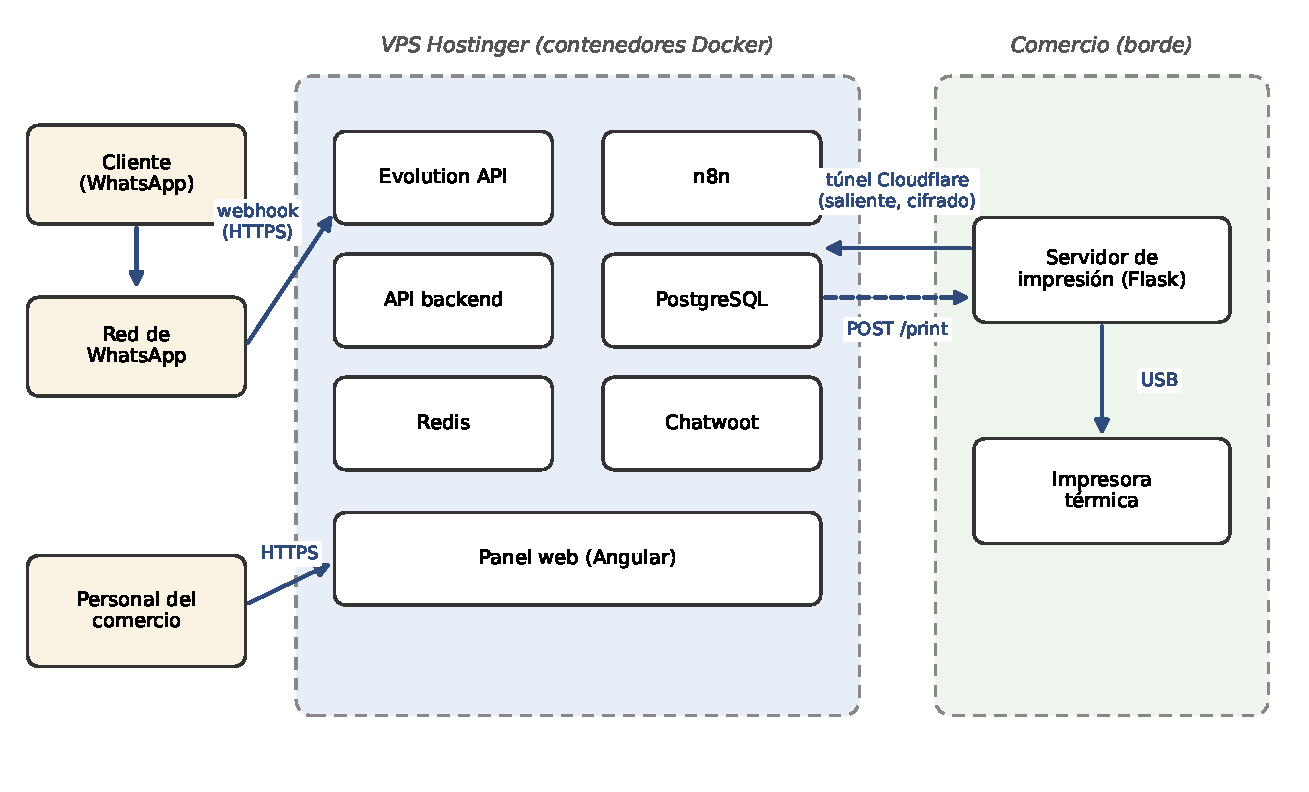
\includegraphics[width=\textwidth]{Figures/topologia_despliegue.pdf}
  \caption{Topología de despliegue del sistema.}
  \label{fig:topologia_despliegue}
\end{figure}

\subsection{Tramos de comunicación}
\label{subsec:tramos}

La conectividad del sistema comprende tres tramos con características distintas.

El primero es el tramo de entrada. La pasarela Evolution API, alojada en el servidor virtual, mantiene la vinculación con la red de WhatsApp y notifica cada mensaje al flujo de n8n mediante peticiones HTTPS, la variante cifrada de HTTP.

El segundo es el tramo interno de la nube. Los servicios contenerizados se comunican entre sí dentro del mismo servidor: el flujo de n8n consulta el catálogo a la API, la API accede a PostgreSQL, y el panel web consume los mismos recursos de la API que utiliza el flujo. Junto a estos servicios opera Chatwoot, una plataforma de gestión de conversaciones que centraliza la bandeja de entrada de WhatsApp. Su integración permite que el personal acceda desde el panel al hilo original de la conversación que dio origen a un pedido, lo que resulta útil ante una interpretación dudosa.

El tercero es el tramo entre la nube y el borde, resuelto mediante el túnel de Cloudflare.

\subsection{Vinculación con el nodo de borde}
\label{subsec:tunel}

La decisión de diseño más relevante de esta capa es el sentido en que se establece la conexión con el comercio. En lugar de exponer el servidor local a Internet mediante la apertura de puertos en el enrutador del negocio, el túnel se establece con una conexión saliente cifrada iniciada desde el propio nodo de borde.

Esta elección tiene tres consecuencias prácticas. La instalación no requiere configurar el equipamiento de red del local, condición decisiva en un comercio sin personal técnico. La red interna del negocio no queda accesible desde el exterior, lo que reduce la superficie de ataque. Y el vínculo se restablece de forma automática tras una interrupción, sin intervención manual.

\subsection{Formato de los mensajes intercambiados}
\label{subsec:payloads}

Los datos que circulan entre los componentes se serializan en formato JSON (del inglés, \textit{JavaScript Object Notation}). El agente de inteligencia artificial produce una estructura fija, que constituye el contrato interno del sistema. El código \ref{lst:pedido_json} muestra su formato.

\begin{lstlisting}[caption={Estructura del pedido devuelto por el agente de interpretación.}, label={lst:pedido_json}]
{
  "is_order": true,
  "items": [
    { "nombre": "Papa", "cantidad": 2, "unidad": "kg" }
  ],
  "aclaraciones": "bien lavadas",
  "productos_no_encontrados": []
}
\end{lstlisting}

El campo \code{is\_order} permite descartar los mensajes que no constituyen un pedido, como saludos o consultas de precio. El campo \code{items} contiene los productos reconocidos, con la denominación exacta del catálogo. El campo \code{aclaraciones} recoge las instrucciones y observaciones del cliente. El campo \code{productos\_no\_\allowbreak encontrados} registra las menciones que no pudieron asociarse a ningún artículo del catálogo, en lugar de descartarlas en silencio. Esta última decisión resultó importante para la trazabilidad: un producto solicitado y no reconocido queda registrado y visible para el personal, en vez de desaparecer del pedido.

El segundo contrato relevante es el del servidor de impresión. El código \ref{lst:print_json} muestra la petición que la API envía al nodo de borde.

\begin{lstlisting}[caption={Petición de impresión enviada al servidor local.}, label={lst:print_json}]
POST /print
X-Printer-Token: <token>

{
  "text": "PEDIDO\n...",
  "printer_name": "Hasar_USB",
  "cut": true,
  "text_size": "double_width"
}
\end{lstlisting}

El campo \code{text} contiene el ticket ya compuesto. Los campos restantes controlan el destino y el formato de impresión: el nombre de la impresora instalada, el corte automático del papel al finalizar y el tamaño de la tipografía. De manera alternativa, la petición admite una dirección IP y un puerto, para el caso en que la impresora se conecte por red. Esa previsión permite trasladar la impresora dentro del local sin modificar el código, tal como se anticipó en el capítulo \ref{Chapter2}.

El servidor de impresión resuelve el envío según la plataforma sobre la que se ejecuta. En Windows utiliza la interfaz de impresión del sistema operativo en modo directo, lo que evita que el controlador reinterprete el contenido y preserva los comandos ESC/POS. En sistemas Linux delega en el sistema de impresión estándar, y ante una impresora de red abre una conexión directa al puerto correspondiente. Esta triple implementación permitió desarrollar y ensayar el componente fuera del entorno del comercio.

%----------------------------------------------------------------------------------------
%	SECTION 4
%----------------------------------------------------------------------------------------

\section{Capa de aplicación y procesamiento}
\label{sec:capa_aplicacion}

Esta capa concentra la interpretación de los pedidos, su validación, la resolución de precios y su persistencia. Es la de mayor complejidad lógica y la que resuelve el problema central del trabajo.

\subsection{Interpretación mediante agentes de inteligencia artificial}
\label{subsec:interpretacion_ia}

La interpretación se implementó como un agente de inteligencia artificial orquestado en n8n. El agente recibe cuatro insumos: el texto agrupado del cliente, sus datos de contacto, el catálogo vigente de productos y la lista de unidades admitidas. Los dos últimos no están fijados en el flujo, sino que se consultan a la API en cada ejecución mediante recursos internos previstos para ese fin. Esta decisión evita la duplicación del catálogo: el personal lo administra desde el panel y el agente siempre opera con la versión actualizada.

El agente cuenta además con memoria de ventana, cuya clave de sesión se construye a partir del teléfono del cliente. De este modo, cada conversación mantiene su contexto de forma independiente.

El comportamiento del agente se define mediante un mensaje de sistema, es decir, la instrucción permanente que delimita su rol y sus reglas antes de recibir cada mensaje del cliente. Su redacción constituyó una parte sustancial del desarrollo, porque de ella dependen tanto la calidad de la interpretación como la estabilidad del formato de salida. El código \ref{lst:prompt_agente} reproduce sus fragmentos más representativos.

\begin{lstlisting}[caption={Fragmentos del mensaje de sistema del agente de interpretación.}, label={lst:prompt_agente}]
# ROL
Sos un asistente para una verduleria. Tu unica tarea es:
1. Determinar si el mensaje del cliente es un pedido de compra.
2. Extraer los productos, cantidades y unidades solicitados.

# CATALOGO
- Para el campo `nombre` en cada item, usa exactamente el nombre
  del catalogo.
- Si el cliente menciona un producto que no esta en el catalogo,
  ponelo en `productos_no_encontrados` (no en `items`).
- Si el cliente usa un apodo o abreviatura que corresponde a un
  producto del catalogo, usa el nombre del catalogo.

# SALIDA
Devolve unicamente el JSON, sin texto adicional ni marcado.
\end{lstlisting}

Tres criterios guiaron esa redacción. El primero es la delimitación estricta del rol, que evita que el agente responda consultas ajenas al pedido. El segundo es la restricción del formato de salida, indispensable para consumir la respuesta de forma programática. El tercero es el tratamiento explícito de los casos ambiguos, que impide que el modelo complete por su cuenta la información faltante.

\subsection{Normalización semántica de productos}
\label{subsec:normalizacion}

Un problema específico del dominio es la variabilidad con que los clientes nombran un mismo producto. Las denominaciones llegan en plural o singular, con diminutivos, con abreviaturas o con errores de tipeo. El sistema debe asociarlas al artículo correcto del catálogo del comercio.

La normalización se resolvió dentro del propio agente, mediante la entrega del catálogo completo como contexto y una instrucción explícita de correspondencia tolerante a variantes. El agente debe utilizar la denominación exacta del catálogo en el campo de salida. Cuando una mención no admite correspondencia razonable, se deriva al campo de productos no encontrados.

Se consideró como alternativa una normalización previa por reglas o por similitud de cadenas. Esa opción se descartó por dos razones. La primera es que las reglas exigen mantenimiento manual ante cada producto nuevo o cada variante no prevista. La segunda es que la similitud de cadenas resuelve mal los casos en que la diferencia es semántica y no ortográfica, como una denominación regional que no comparte raíz con el nombre del catálogo. La estrategia adoptada traslada esa responsabilidad al modelo, que dispone del catálogo completo y del contexto del mensaje.

\subsection{Recursos de la interfaz de programación}
\label{subsec:api}

La API se organizó por recursos, con un prefijo común y un archivo de rutas por entidad. En la tabla \ref{tab:endpoints} se resumen los grupos de recursos y su mecanismo de acceso.

\begin{table}[htbp]
  \centering
  \caption{Grupos de recursos de la interfaz de programación.}
  \label{tab:endpoints}
  \small
  \begin{tabular}{l l l}
    \toprule
    \textbf{Recurso}         & \textbf{Función}             & \textbf{Acceso}             \\
    \midrule
    \code{/auth}             & Autenticación de personas    & Público                     \\
    \code{/pedidos}          & Creación, consulta y edición & Clave de servicio o testigo \\
    \code{/productos}        & Catálogo de productos        & Testigo (catálogo: clave)   \\
    \code{/unidades}         & Unidades de medida           & Testigo (catálogo: clave)   \\
    \code{/categorias}       & Categorías de productos      & Testigo, rol administrador  \\
    \code{/clientes}         & Clientes y listas de precios & Testigo                     \\
    \code{/precios\_default} & Precios generales            & Testigo                     \\
    \code{/print-logs}       & Historial de impresiones     & Testigo                     \\
    \code{/metricas}         & Indicadores de operación     & Testigo                     \\
    \code{/usuarios}         & Usuarios del sistema         & Testigo, rol administrador  \\
    \bottomrule
  \end{tabular}
\end{table}

La creación de un pedido desde el flujo automático y su creación desde el panel se resolvieron con recursos distintos, aunque compartan la lógica de persistencia. La separación responde a que difieren en su origen, en su mecanismo de autenticación y en la validación aplicada: el flujo entrega productos ya normalizados por el agente, mientras que el panel recibe datos ingresados por una persona.

\subsection{Modelo de datos}
\label{subsec:modelo_datos}

La persistencia se resolvió sobre PostgreSQL, con acceso mediante el ORM Prisma. El esquema se controla por migraciones versionadas, lo que permite reproducir la estructura de la base en cualquier entorno. En la figura \ref{fig:der} se presenta el diagrama entidad-relación con las entidades principales.

\begin{figure}[htbp]
  \centering
  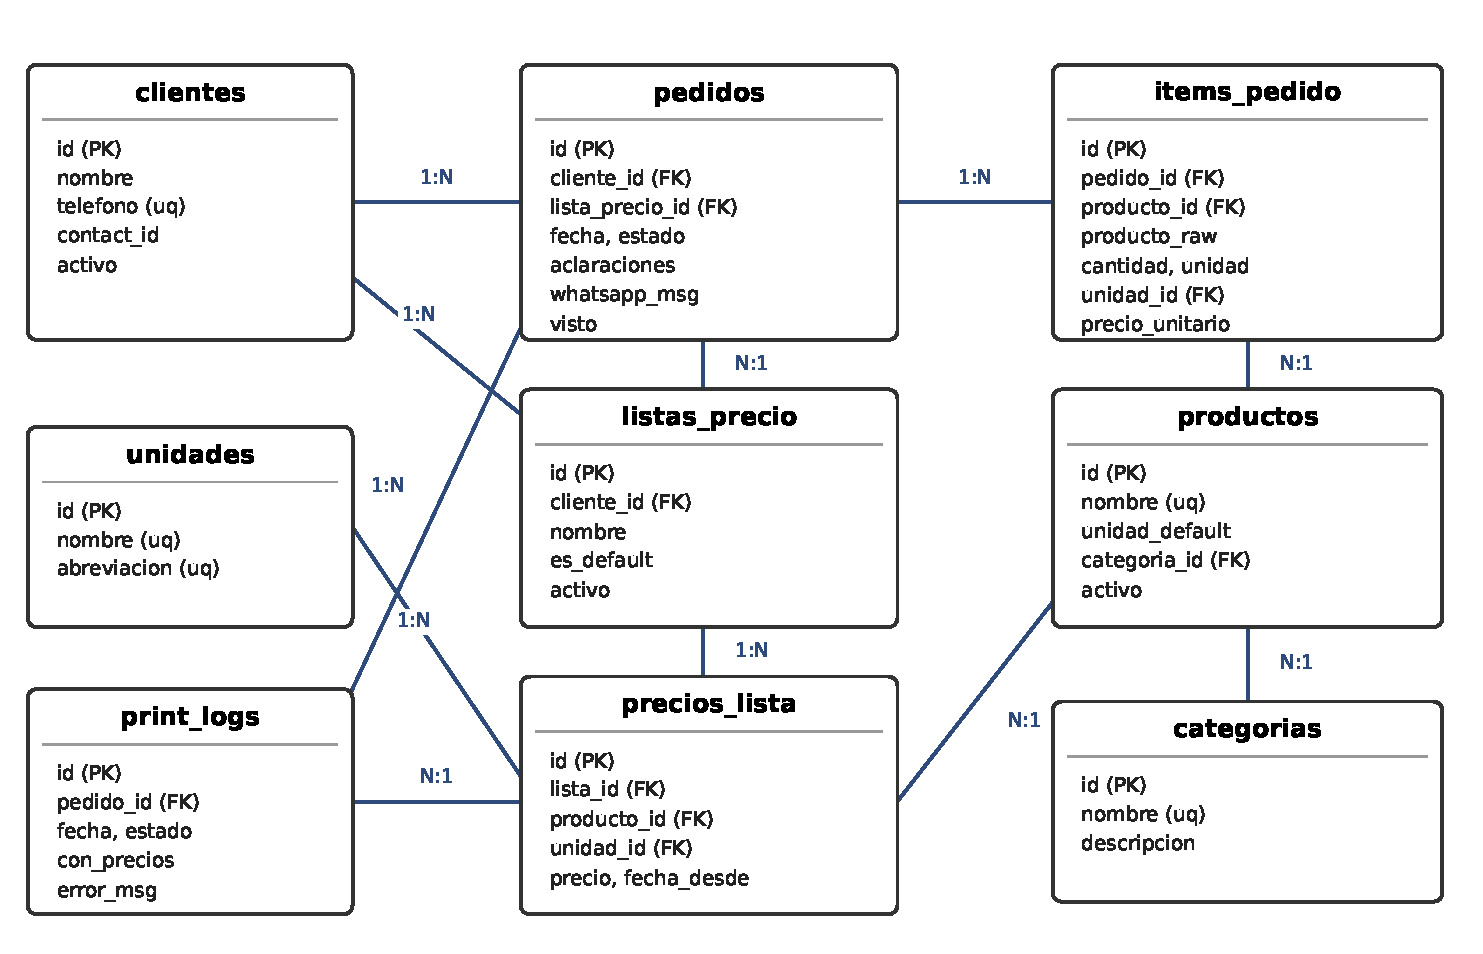
\includegraphics[width=\textwidth]{Figures/der_base_datos.pdf}
  \caption{Diagrama entidad-relación de la base de datos.}
  \label{fig:der}
\end{figure}

El núcleo del modelo lo constituyen las entidades \code{clientes}, \code{pedidos} e \code{items\_\allowbreak pedido}. Un cliente se identifica por su teléfono, con restricción de unicidad, y acumula sus pedidos. Cada pedido registra la fecha, el estado, las aclaraciones y el mensaje original recibido por WhatsApp. Este último campo resulta clave para la trazabilidad, ya que permite contrastar el pedido estructurado contra el texto que le dio origen.

La entidad \code{items\_pedido} presenta una particularidad de diseño. Junto a la referencia al producto del catálogo conserva un campo con la denominación original empleada por el cliente. Cuando la referencia al catálogo queda vacía, el ítem corresponde a un producto no reconocido. Esos ítems no se descartan: se conservan, se imprimen en una sección separada del ticket y se destacan visualmente en el panel para que el personal decida cómo proceder.

El estado del pedido se modeló como una enumeración con cuatro valores: recibido, en preparación, listo y entregado. La enumeración impide que la base admita estados no previstos y ordena el recorrido operativo del pedido dentro del comercio.

El modelo contempla además dos operaciones propias del uso real. La primera es la fusión de pedidos: cuando un cliente envía un pedido complementario poco después del primero, el personal puede unificarlos desde el panel. El modelo conserva la referencia al pedido resultante y la marca temporal de la operación, lo que permite deshacerla sin pérdida de información. La segunda es la marca de pedido visto, que distingue los pedidos ya revisados por el personal de los que aún esperan atención.

\subsection{Resolución de precios}
\label{subsec:precios}

La gestión de precios responde a una característica del negocio: no todos los clientes pagan lo mismo. El comercio atiende tanto a consumidores finales como a otros comercios, con condiciones diferenciadas.

El modelo resuelve esa necesidad mediante listas de precios. Cada cliente puede tener varias listas, y una de ellas se designa como predeterminada. El precio de un ítem se resuelve por orden de prioridad: primero la lista indicada de forma explícita en el pedido, luego la lista predeterminada del cliente y, por último, el precio general del catálogo. Los precios incorporan además vigencia temporal, con fechas de inicio y de fin, lo que permite conservar el histórico sin perder el valor aplicado en cada momento.

Un diseño alternativo, con un único precio por cliente y producto, habría resultado más simple. Se descartó porque impide representar acuerdos comerciales distintos para un mismo cliente, como una condición mayorista y otra minorista, y porque no conserva el histórico de precios necesario para las métricas de facturación.

\subsection{Generación del ticket}
\label{subsec:ticket}

El ticket no se almacena en la base de datos, sino que se compone en el momento de la impresión a partir de los ítems del pedido y de sus aclaraciones. Esta decisión evita la duplicación de información y garantiza que una reimpresión refleje el estado actual del pedido, incluidas las correcciones realizadas por el personal.

La impresión admite dos variantes, con precios y sin precios. El flujo automático imprime sin precios, porque el ticket cumple allí la función de orden de armado. Desde el panel, en cambio, el personal elige la variante al momento de imprimir, según entregue el comprobante al cliente o lo destine al armado interno.

Cada intento de impresión se registra en una entidad específica, con su resultado, la variante utilizada y el mensaje de error en caso de falla. Ese registro cumple dos funciones: permite auditar qué se imprimió y cuándo, y habilita el seguimiento de los errores hasta su resolución. Los pedidos con impresión fallida se destacan en el panel y permanecen señalados hasta que el personal los marca como resueltos, de modo que una falla de la impresora no derive en un pedido sin atender.

%----------------------------------------------------------------------------------------
%	SECTION 5
%----------------------------------------------------------------------------------------

\section{Interfaz de usuario y visualización}
\label{sec:interfaz}

El sistema presenta dos interfaces hacia el personal del comercio: el ticket impreso y el panel web de control.

\subsection{El ticket impreso}
\label{subsec:ticket_impreso}

El ticket es la salida física del sistema y el insumo directo para el armado del pedido. Su formato es fijo. Incluye un encabezado con los datos del cliente, la lista de productos con cantidades y unidades, una sección separada para los productos no reconocidos, un espacio para las aclaraciones y la fecha y hora del pedido. En la figura \ref{fig:ticket} se muestra un ticket generado por el sistema.

\begin{figure}[htbp]
  \centering
  % [PENDIENTE: reemplazar por la fotografía del ticket impreso, con datos de ejemplo.]
  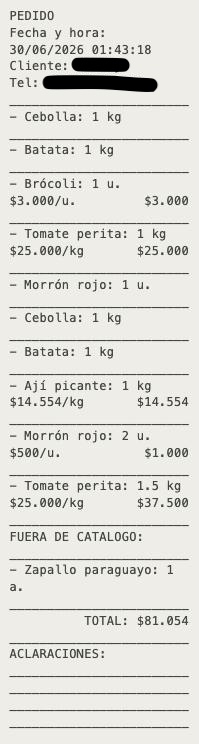
\includegraphics[width=0.45\textwidth]{Figures/ticket_impreso.jpeg}
  \caption{Ticket generado por el sistema e impreso en el comercio.}
  \label{fig:ticket}
\end{figure}

El diseño del ticket estuvo condicionado por el medio. El ancho útil del papel es de ochenta milímetros, lo que limita la cantidad de caracteres por línea y obliga a priorizar la información. Por ese motivo, el servidor de impresión admite distintos tamaños de tipografía, que se aplican mediante comandos ESC/POS. Los datos que el personal necesita leer a distancia, en particular el nombre del cliente, se imprimen en tamaño ampliado, mientras que el detalle de los productos se mantiene en tamaño normal para aprovechar el ancho disponible.

\subsection{El panel web de control}
\label{subsec:panel}

El panel se desarrolló con Angular y la biblioteca de componentes Angular Material. Concentra la operación diaria y la administración del sistema. El acceso está protegido por autenticación, y las vistas de administración quedan restringidas según el rol de la persona que ingresa.

\subsubsection{Tablero principal}

El tablero es la vista de entrada al sistema y resume el estado de la operación del día. En la figura \ref{fig:panel_dashboard} se presenta esa vista.

\begin{figure}[htbp]
  \centering
  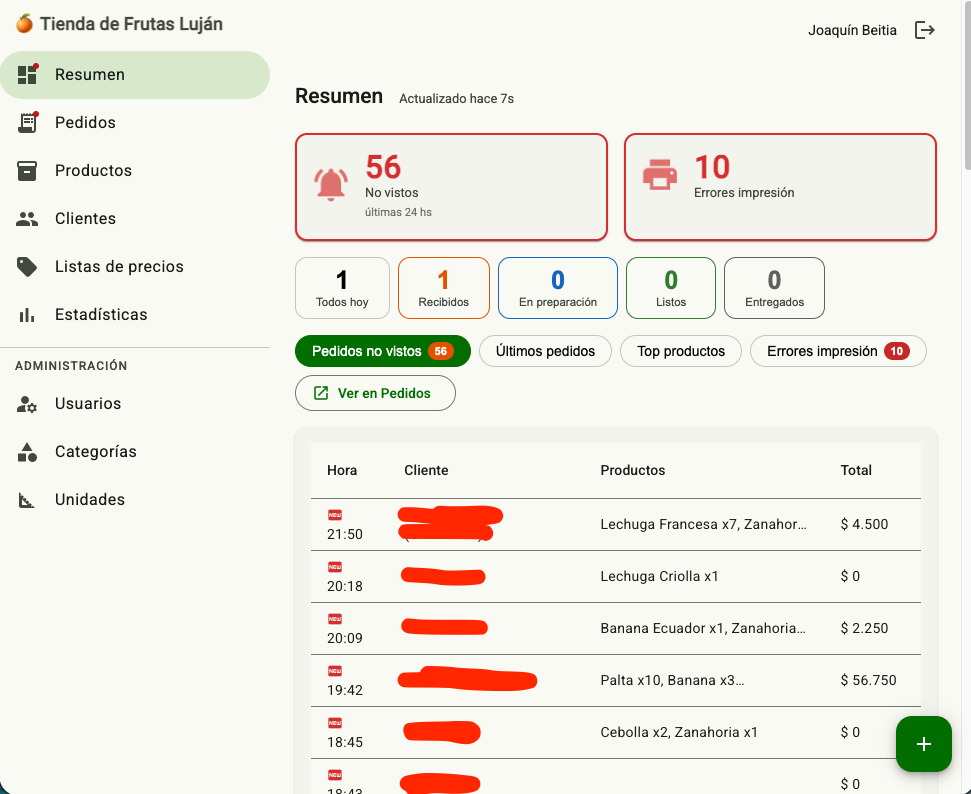
\includegraphics[width=\textwidth]{Figures/panel_dashboard.png}
  \caption{Tablero principal del panel de control.}
  \label{fig:panel_dashboard}
\end{figure}

El tablero agrupa cuatro bloques de información: los pedidos aún no revisados por el personal, los pedidos recibidos en los últimos minutos, los productos más solicitados en el día y los pedidos con errores de impresión pendientes de resolución. Cada bloque enlaza con la vista de pedidos, con los filtros ya aplicados, de modo que una alerta deriva de forma directa en la acción correspondiente.

\subsubsection{Gestión de pedidos}

La vista de pedidos es la de mayor uso durante la jornada. Permite filtrar por estado, por rango de fechas, por pedidos no vistos y por errores de impresión. En la figura \ref{fig:panel_pedidos} se muestra el listado.

\begin{figure}[htbp]
  \centering
  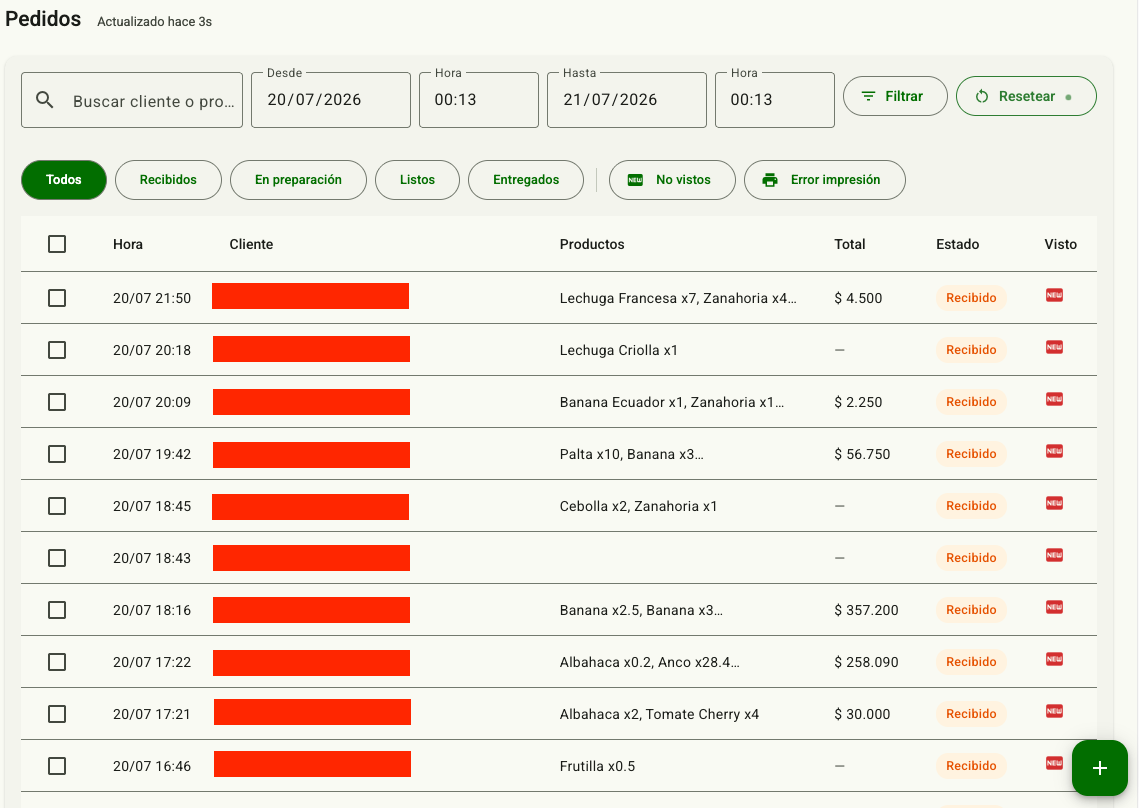
\includegraphics[width=\textwidth]{Figures/panel_pedidos.png}
  \caption{Listado de pedidos con sus filtros de búsqueda.}
  \label{fig:panel_pedidos}
\end{figure}

El listado admite operaciones sobre varios pedidos a la vez, como el cambio de estado o la marca de revisado, pensadas para los momentos de mayor demanda. El detalle de cada pedido se abre en un diálogo que concentra la operación individual, según se observa en la figura \ref{fig:panel_detalle}.

\begin{figure}[htbp]
  \centering
  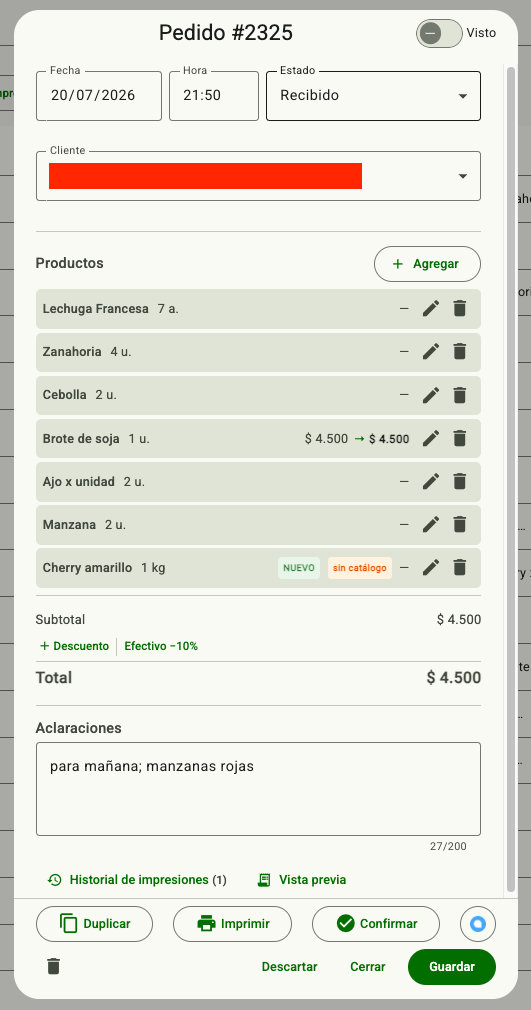
\includegraphics[width=0.55\textwidth]{Figures/panel_detalle_pedido.png}
  \caption{Detalle de un pedido, con edición de ítems y acceso al mensaje original.}
  \label{fig:panel_detalle}
\end{figure}

Desde ese diálogo, el personal puede corregir las cantidades y las unidades, agregar o quitar ítems, consultar el mensaje original recibido por WhatsApp, acceder al hilo de la conversación e imprimir o reimprimir el pedido. Los ítems que no pudieron asociarse al catálogo se destacan de forma visual, lo que dirige la atención del personal hacia los casos que requieren decisión.

\subsubsection{Administración del catálogo y de los precios}

El catálogo de productos, sus categorías y las unidades de medida se administran desde el panel. Esta gestión resulta crítica para el funcionamiento del sistema, ya que el catálogo es el insumo que el agente utiliza para normalizar las denominaciones. Un producto ausente del catálogo se traduce de inmediato en ítems no reconocidos en los pedidos.

\begin{figure}[htbp]
  \centering
  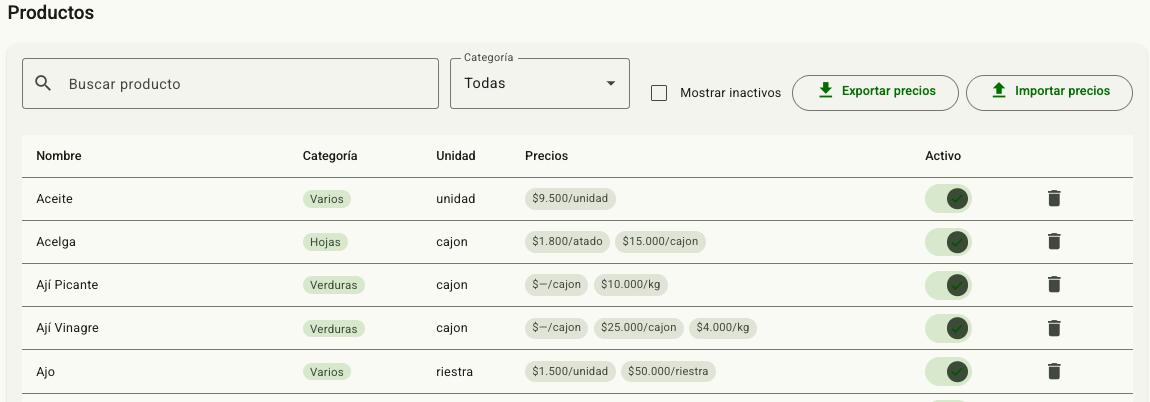
\includegraphics[width=\textwidth]{Figures/panel_productos.png}
  \caption{Administración del catálogo de productos.}
  \label{fig:panel_productos}
\end{figure}

La administración de precios se resolvió en una vista específica, con el listado de listas del cliente a un lado y la tabla de precios editable al otro. En la figura \ref{fig:panel_precios} se presenta esa vista.

\begin{figure}[htbp]
  \centering
  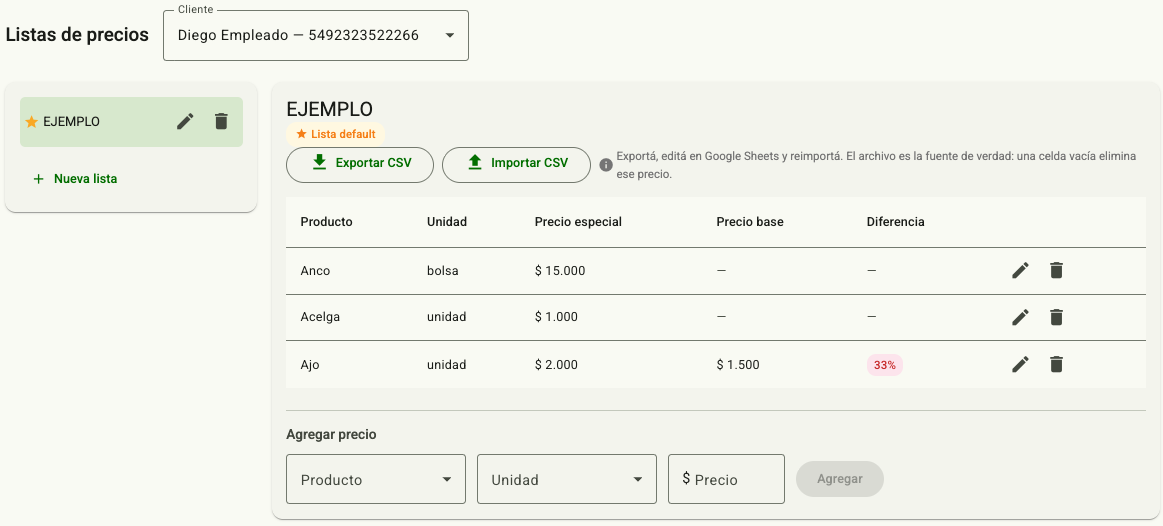
\includegraphics[width=\textwidth]{Figures/panel_listas_precios.png}
  \caption{Administración de las listas de precios de un cliente.}
  \label{fig:panel_precios}
\end{figure}

\subsubsection{Métricas de operación}

Las métricas se representan con la biblioteca Chart.js. La vista incluye el tráfico de pedidos por día y hora, la evolución de la facturación por producto y la distribución por categoría. En la figura \ref{fig:panel_estadisticas} se muestra esa vista.

\begin{figure}[htbp]
  \centering
  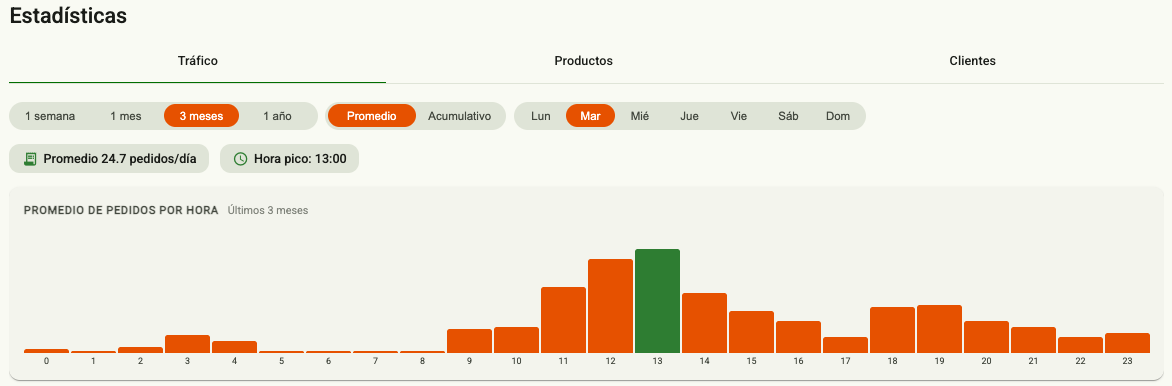
\includegraphics[width=\textwidth]{Figures/panel_estadisticas.png}
  \caption{Vista de métricas de operación del comercio.}
  \label{fig:panel_estadisticas}
\end{figure}

La consulta admite distintos rangos temporales, y la granularidad de la serie se ajusta de forma automática al rango solicitado: diaria hasta una semana, semanal hasta tres meses y mensual para períodos mayores. Este ajuste evita gráficos ilegibles por exceso de puntos. El tráfico por día y hora resultó de utilidad directa para el negocio, ya que expone los momentos de mayor demanda y permite anticipar la asignación de personal.

%----------------------------------------------------------------------------------------
%	SECTION 6
%----------------------------------------------------------------------------------------

\vspace{50em}
\section{Seguridad del sistema}
\label{sec:seguridad}

La seguridad se abordó en tres frentes: el control de acceso, la protección de las comunicaciones y la integridad de los datos.

\subsection{Autenticación y control de acceso}
\label{subsec:autenticacion}

El sistema distingue dos tipos de consumidores, con mecanismos de autenticación distintos. Las personas acceden al panel con credenciales y obtienen un testigo de sesión. Los servicios internos, como el flujo de n8n, no disponen de una sesión de usuario y se autentican con una clave de servicio. En la figura \ref{fig:auth} se representan ambos mecanismos.

\begin{figure}[htbp]
  \centering
  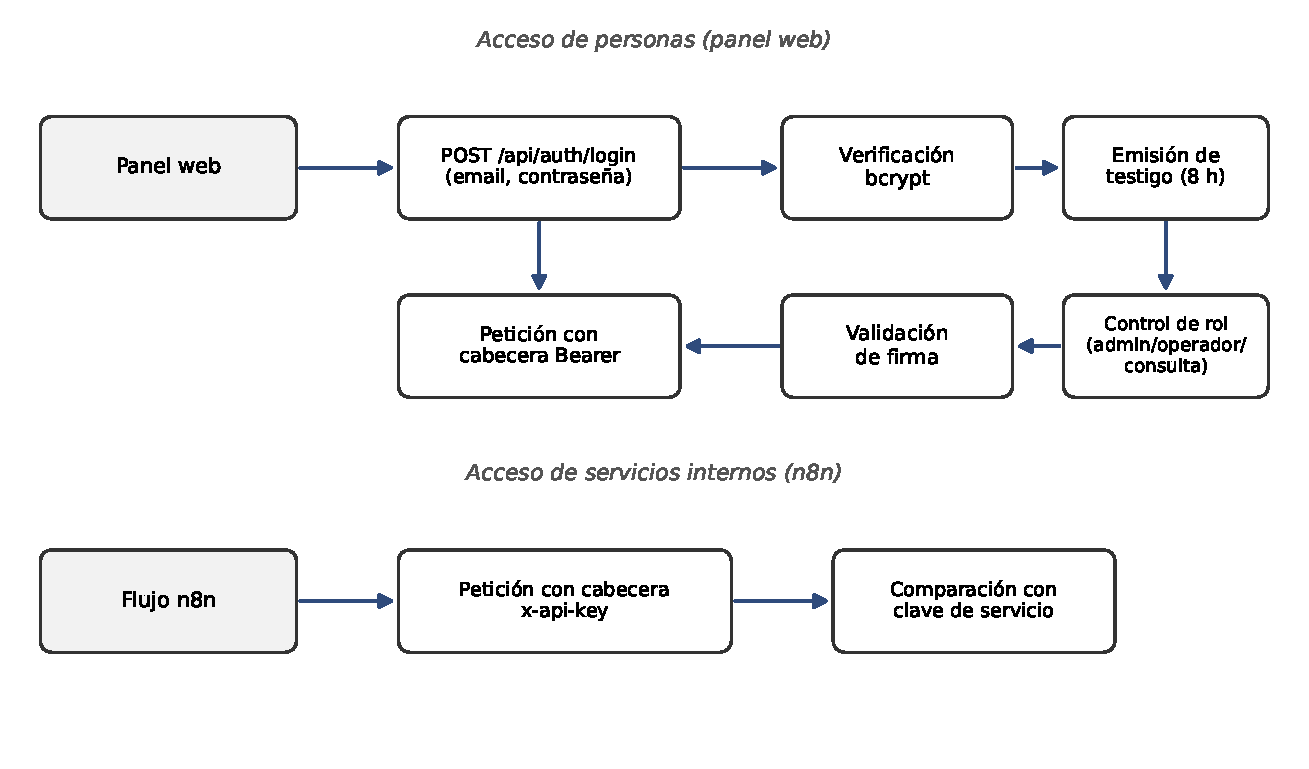
\includegraphics[width=\textwidth]{Figures/flujo_autenticacion.pdf}
  \caption{Mecanismos de autenticación para personas y para servicios internos.}
  \label{fig:auth}
\end{figure}

Las contraseñas se almacenan cifradas mediante una función de derivación diseñada para ese fin, de modo que la base no conserva las claves en texto plano. Tras una validación exitosa, el sistema emite un testigo firmado con vigencia de ocho horas, que el panel adjunta en cada petición posterior. La vigencia se ajustó a la duración de una jornada comercial, lo que evita tanto la reautenticación durante el turno como la persistencia indefinida de una sesión abierta.

La autorización se implementó por roles. El sistema define tres: administrador, con acceso total; operador, restringido a la operación de pedidos; y consulta, limitado a la lectura. La verificación se resuelve con un componente intermedio que valida el rol antes de ejecutar cada operación, lo que centraliza la regla y evita repetirla en cada recurso. El panel replica esa restricción en sus rutas, de modo que las vistas de administración no resultan accesibles para los roles que no corresponden.

Los recursos internos, como la consulta del catálogo y la creación de pedidos desde el flujo, admiten únicamente la clave de servicio. El recurso de impresión constituye una excepción deliberada, ya que acepta ambas formas de autenticación: la clave de servicio para la impresión automática y el testigo de sesión para la reimpresión desde el panel.

\subsection{Protección de las comunicaciones}
\label{subsec:proteccion_comunicaciones}

Todo el tráfico externo circula cifrado. La pasarela de mensajería entrega los mensajes por HTTPS y el vínculo entre la nube y el borde se resuelve mediante el túnel descripto en la sección \ref{subsec:tunel}, cuya conexión saliente cifrada evita exponer puertos entrantes en la red del comercio. El servidor de impresión exige, además, un testigo propio en cada petición, de modo que la sola llegada al servicio no habilita la impresión.

\subsection{Gestión de credenciales e integridad de los datos}
\label{subsec:credenciales}

Las credenciales de los servicios externos y las claves de firma se gestionan mediante variables de entorno, fuera del código fuente. Los archivos que las contienen quedan excluidos del control de versiones, y el repositorio conserva únicamente valores de ejemplo. Este criterio evita que una credencial operativa quede registrada en el historial del repositorio.

En cuanto a la integridad, el modelo de datos define restricciones de unicidad sobre los campos que identifican a clientes, productos y unidades, y relaciones con integridad referencial entre las entidades. La eliminación de un pedido arrastra sus ítems y sus registros de impresión, lo que evita la persistencia de datos huérfanos. Redis se reservó de manera estricta para información temporal, de modo que una falla en la capa en memoria no compromete los registros del negocio.